% DOCUMENT CLASS %
\documentclass[a4paper, 12pt]{extarticle}   % for A4 Paper, 12pt fontsize and article spacing
\usepackage[left=1.5cm,right=1.5cm,top=2cm,bottom=2cm]{geometry}    % Make the page a little bigger

% PACKAGES%
\usepackage{amsfonts}   % For a basic mathfont (many will be replaced by stix)
\usepackage{amsmath}    % For basic math symbols
\usepackage{bbm}        % For \mathbbm (better version of \mathbb)
\usepackage{mathrsfs}   % For \mathscr
\usepackage{hyperref}   % For footnotes
\usepackage{csquotes}   % For \textquote{}
\usepackage{IEEEtrantools}  % For better alignments
\usepackage{tikz}   % For a macro
\usetikzlibrary{arrows.meta, positioning, calc}	% For protocol diagrams
\usepackage{listings} % For code
\usepackage{xcolor}   % For ... code
\usepackage{microtype}  % For better paragraph formatting
\usepackage{amsthm}   % For custom environments

% FONT CONFIGURATION %
\usepackage[T1]{fontenc}
\usepackage{palatino}

% BASIC SETS %
\newcommand*{\R}{\mathbbm R}    % Set of real numbers
\newcommand*{\N}{\mathbbm N}    % Set of natural numbers (beginning at 0)
\newcommand*{\Z}{\mathbbm Z}    % Set of integers
\newcommand*{\Q}{\mathbbm Q}    % Set of rational numbers

% MACROS %
\newcommand*{\qedbox}{\null\nobreak\hfill\ensuremath{\square}} % Macro for a QED-Box
% for a funny ¯\_(ツ)_/¯-Emoji
\newcommand{\shrug}[1][]{%
    \begin{tikzpicture}[baseline,x=0.8\ht\strutbox,y=0.8\ht\strutbox,line width=0.125ex,#1]
    \def\arm{(-2.5,0.95) to (-2,0.95) (-1.9,1) to (-1.5,0) (-1.35,0) to (-0.8,0)};
    \draw \arm;
    \draw[xscale=-1] \arm;
    \def\headpart{(0.6,0) arc[start angle=-40, end angle=40,x radius=0.6,y radius=0.8]};
    \draw \headpart;
    \draw[xscale=-1] \headpart;
    \def\eye{(-0.075,0.15) .. controls (0.02,0) .. (0.075,-0.15)};
    \draw[shift={(-0.3,0.8)}] \eye;
    \draw[shift={(0,0.85)}] \eye;
    % draw mouth
    \draw (-0.1,0.2) to [out=15,in=-100] (0.4,0.95); 
    \end{tikzpicture}
}

% BASIC CONFIGURATION %
\pagestyle{plain}
\allowdisplaybreaks

% CODE CONFIGURATIONS %
\definecolor{codepurple}{HTML}{7f0055}
\definecolor{comment}{RGB}{0,128,0}
\definecolor{number}{RGB}{9,136,90}
\definecolor{string}{RGB}{163,21,21}

\lstset{
    language=python,
    emph={*, do, od, for, if, fi, then, else, to, def, in, forall, exists},
    firstnumber=1,
    basicstyle=\small\ttfamily,
    breaklines=true,
    breakatwhitespace=false,
    frame=tb,
    captionpos=b,
    %float=t,
    %floatplacement=t,
    abovecaptionskip=0.5cm,
    numbers=left,
    numberstyle=\tiny,
    keywordstyle=\bfseries\color{codepurple},
    emphstyle=\bfseries\color{codepurple},
    mathescape=true,
    keepspaces=true,
    showspaces=false,
    showstringspaces=false,
    showtabs=false,
    stringstyle=\color{string},
    commentstyle=\itshape\color{comment},
    upquote=true,
    texcl=true
}

% EXERCISE ENVIRONMENT %
\theoremstyle{definition}
\newtheorem{exercise}{Exercise}[section]
\setcounter{section}{1} % Don't use \section and this works naturally

% TITLE CONFIGURATION %
\newcommand{\ex}{0}

\title{Data Visualization \\ \small Exercise Sheet \ex}
\date{Winter Term 2025/26}
\author{
    Henri Heyden \\%
    \small stu240825%
    \and
    Julia Schröder \\%
    \small stu252018%
    \and
    Rebecca Ziebell \\%
    \small stu250567%
}


\renewcommand{\ex}{3}
\setcounter{section}{\ex}

\begin{document}
    \maketitle

    \begin{exercise}[Encode the Following Values in 20 Different Ways] \hfill
        \begin{itemize}
            \item[a)] See \autoref{fig:1a}.
                \begin{figure}[t]
                    \centering
                    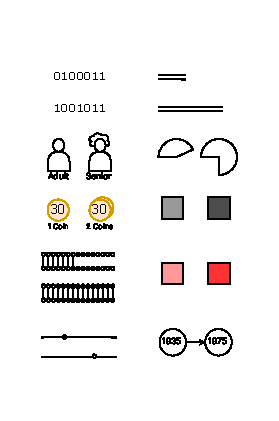
\includegraphics[width=0.6\textwidth]{1a.pdf}
                    \caption{The values \emph{35} and \emph{75} visually encoded in 10 different ways.}
                    \label{fig:1a}
                \end{figure}
            \item[b)] See \autoref{fig:1b}.
                \begin{figure}[t]
                    \centering
                    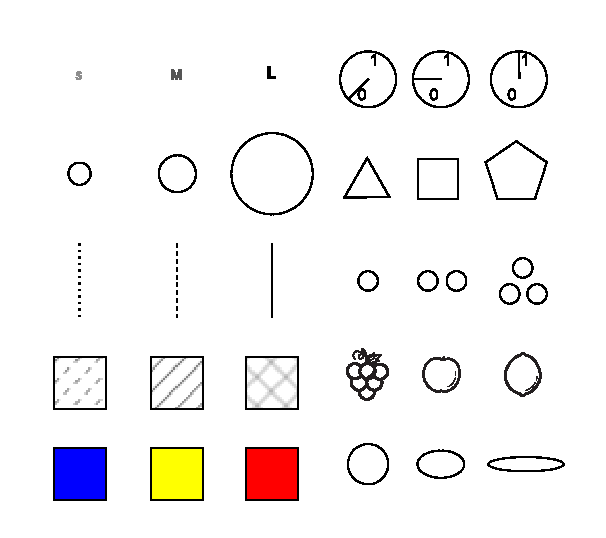
\includegraphics[width=0.6\textwidth]{1b.pdf}
                    \caption{The values \emph{small}, \emph{medium}, and \emph{large} visually encoded in 10 different ways.}
                    \label{fig:1b}
                \end{figure}
        \end{itemize}
    \end{exercise}

    \begin{exercise}[Data Encoding Terms] \hfill
        \begin{itemize}
            \item Marks

            They represent information, like items or connections between items, in simple geometrical shapes.
            Examples for marks could be points, lines, areas or figures.

            \item Channels

            Channels control the visuals of marks and they can be varied to encode data, such as positions, lenght
            color, shape or size.

            \item Expressiveness

            Expressiveness is an important aspect because it refers to whether a visual encoding correctly represents
            all the important aspects of the relevant data, without any incorrect information.

            \item Effectiveness

            This principle describes that the most important information should be highlighted 
            with the most noticable channels, so that the importance of the data is clearly visible.

            \item Separability

            It describes how independently two channels can be perceived. If channels are separable,
            changing one does not affect how the other is seen.

            \item Integrality

            This principle describes when two channels are perceived together as a single
            combined feature. Changing one channel naturally affects the perception of the other.
        \end{itemize}

    \end{exercise}

    \begin{exercise}[Effectiveness]
        
        Ordered by effectiveness:

        \noindent
        Saturation $\rightarrow$ Luminance $\rightarrow$ Area $\rightarrow$ Length $\rightarrow$ Position
    \end{exercise}

    \begin{exercise}[Car Dataset with Altair]
        \begin{centering}
            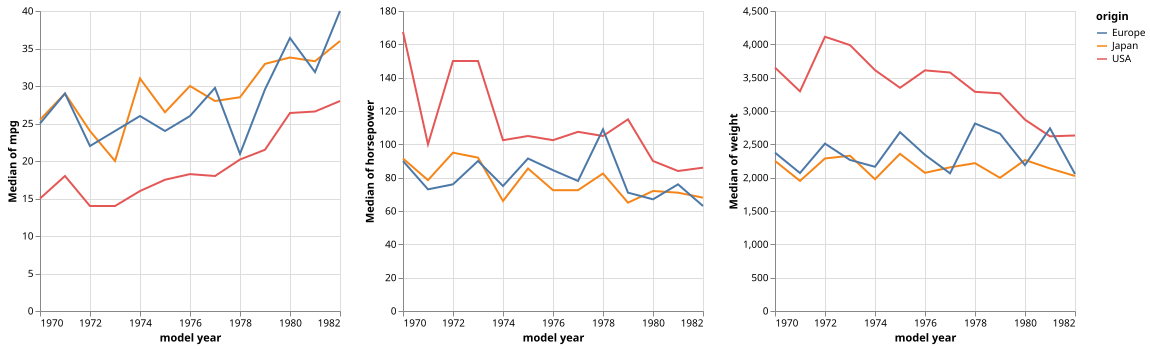
\includegraphics[0.9\textwidth]{mpg_hp_weight.svg}
        \end{centering}

        During exploration of the dataset I found what I already anticipated: The miles per gallon (mpg) rose over the years. Also cars from the USA were less efficient, heavier and had more horsepowers. Interestingly the median weight roughly stayed the same for European and Japanese cars and even fell over the years for cars from the US, completely in contrast to my impression that cars got on average larger in recent years.

        \begin{centering}
            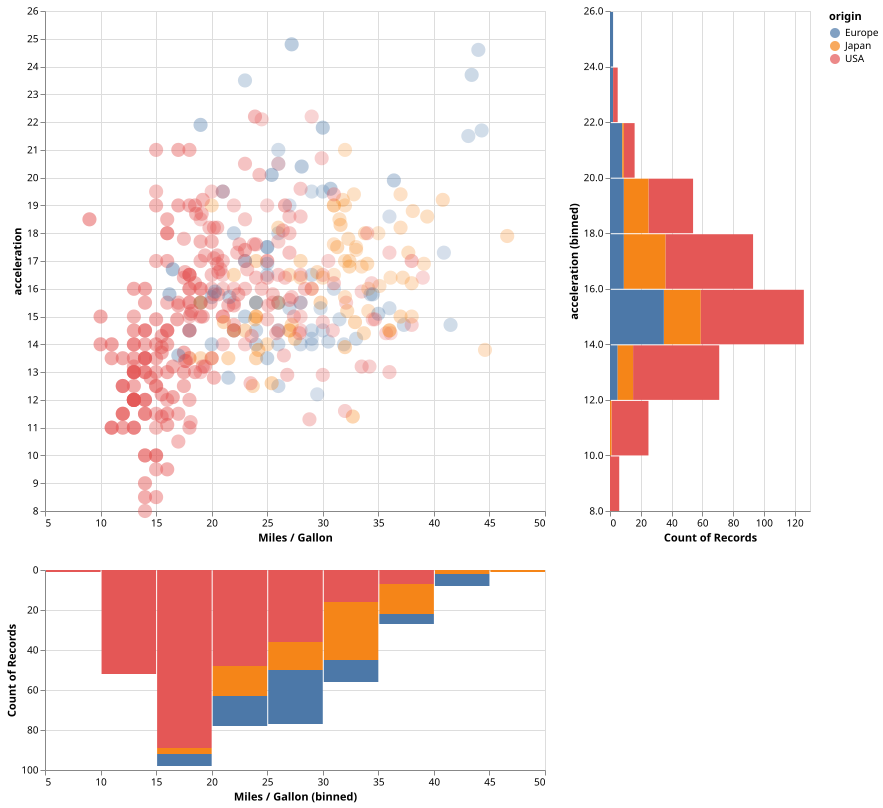
\includegraphics[0.9\textwidth]{mpg_origin_accel.svg}
        \end{centering}

        This chart shows acceleration against mpg, weight and origin. The weight is shown as the opacity of the circles, heavier being more opaque (for some reason Altair did not include this in the legend).
        
        \begin{centering}
            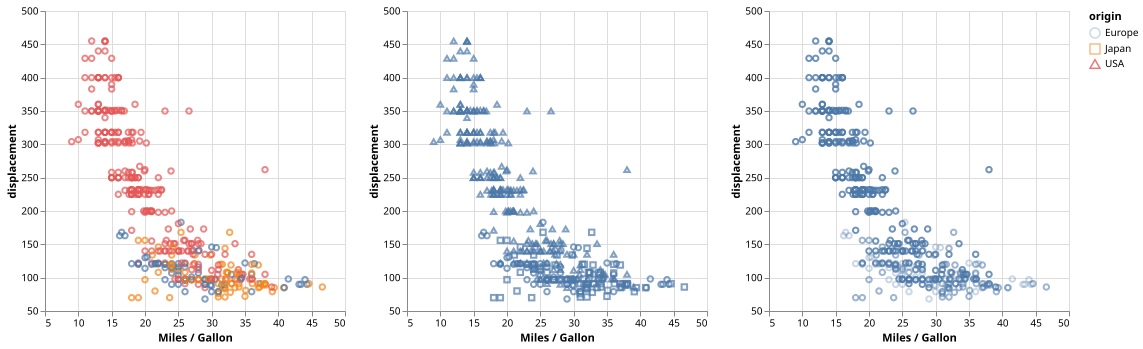
\includegraphics[0.9\textwidth]{encodings.svg}
        \end{centering}

        In my opinion color conveys the origin of a car most clearly and still works well even in very crowded areas on the graph. Shape also creates the right intuition but becomes completely undiscernable in crowded areas. Opacity is definetely bad as it both creates a wrong idea of a continuous scale and is also hard to discern. Probably the worst is size, which isn't shown here but has the same problems as opacity while also completely cluttering the graph.

        These encodings might be suited for other tasks but I would avoid all but the first two for nominal data.
    \end{exercise}
\end{document}
